%% Direttive TeXworks:
% !TeX root = ../maltoni_niccolo_tesi.tex
% !TEX encoding = UTF-8 Unicode
% !TEX program = arara
% !TEX TS-program = arara
% !TeX spellcheck = it-IT

%% Direttive Arara:
% arara: pdflatex: { shell: yes, synctex: yes, action: batchmode, options: "-halt-on-error -file-line-error-style" }
% arara: frontespizio
% arara: biber
% arara: pdflatex: { shell: yes, synctex: yes, action: batchmode, options: "-halt-on-error -file-line-error-style" }
% arara: pdflatex: { shell: yes, synctex: yes, action: nonstopmode, options: "-halt-on-error -file-line-error-style" }

\chapter{Introduzione}\label{ch:intro}

    \section{Alchemist}\label{sec:alchemist}
        Alchemist~\cite{alchemistWeb, alchemist2013} è un meta-simulatore estendibile completamente \engEmph{open-source} che esegue su \engEmph{Java~Virtual~Machine} (JVM), nato all'interno del'Università di Bologna e distribuito su licenza GNU GPLv3+ con \engEmph{linking exception}; il codice è reperibile su GitHub\footnote{\url{https://github.com/AlchemistSimulator/Alchemist}}\label{fn:gh}, dove chiunque fosse interessato può collaborare sviluppando nuove estensioni, migliorando funzionalità esistenti e risolvendo possibili bug.

        \subsection{Introduzione ad Alchemist}\label{sub:introAlchemist}
            In generale, una \emph{simulazione}~\cite{des3} è una riproduzione del modo di operare di un sistema o un processo del mondo reale nel tempo.
            L'imitazione del processo del mondo reale è detta \emph{modello}; esso risulta essere una riproduzione più o meno semplificata del mondo reale, che viene aggiornata ad ogni passo di esecuzione della simulazione.

            Alchemist rientra nell'archetipo dei simulatori ad eventi discreti (DES)~\cite{des, des2}: gli eventi sono strettamente ordinati e vengono eseguiti uno alla volta, mentre il tempo viene fatto avanzare parallelamente ad ogni passo (detto \engEmph{tick}).
            L'idea dietro al progetto è quello di riuscire ad avere un framework di simulazione il più possibile generico, in grado di simulare sistemi di tipologia e complessità diverse, mantenendo le prestazioni dei simulatori non generici (come ad esempio quelli impiegati in ambito chimico~\cite{gillespie1976}).

            Per perseguire questo obiettivo, la progettazione dell'algoritmo è partita dallo studio del lavoro di Gillespie del 1977~\cite{gillespie1977} e di altri scienziati nell'ambito della simulazione chimica. Nonostante siano presenti algoritmi in grado di eseguire un numero di reazioni addirittura in tempo costante, la scelta dell'algoritmo è infine ricaduta su una versione migliorata dell'algoritmo SSA di Gillespie, il Next Reaction Method~\cite{nextReactionMethod} di Gibson e Bruck: ad ogni passo di simulazione, esso è in grado di selezionare la reazione successiva in tempo costante e richiede un tempo logaritmico per aggiornare le strutture dati interne al termine dell'esecuzione dell'evento.

        % \subsection{Architettura di Alchemist}\label{sub:architettura}
            % TODO analizza architettura Alchemist e separala dal modello

        \subsection{Astrazioni e modello di Alchemist}\label{sub:modello}
            Il modello di astrazione di Alchemist è ispirato dal lavoro della comunità scientifica nell'ambito dei simulatori a scopo di ricerca chimica e, dunque, ne riprende la nomenclatura, seppur con alcune libertà per favorire
            Le entità (visibile in \figurename~\vref{fig:model}) su cui lavora sono le seguenti:

            \begin{description}
                \item[\engEmph{Molecule}\label{itm:mol}]
                    Una \emph{Molecola} rappresenta il nome dato ad un particolare dato all'interno di un \emph{Nodo}, del quale ne astrae parte dello stato.

                    Un parallelismo con la programmazione imperativa vedrebbe la \emph{Molecola} come un'astrazione del nome di una variabile.

                \item[\engEmph{Concentration}\label{itm:conc}]
                    La \emph{Concentrazione} di una \emph{Molecola} è il valore associato alla proprietà rappresentata dalla \emph{Molecola}.

                    Mantenendo il parallelismo con la programmazione imperativa, la \emph{Concentrazione} rappresenterebbe il valore della variabile.

                \item[\engEmph{Node}\label{itm:node}]
                    Il \emph{Nodo} è un contenitore di \emph{Molecole} e \emph{Reazioni} che risiede all'interno di un \emph{Ambiente} e che astrae una singola entità.

                \item[\engEmph{Environment}\label{itm:env}]
                    L'\emph{Ambiente} è l'astrazione che rappresenta lo spazio nella simulazione ed è l'entità che contiene i nodi.

                    Esso è in grado di fonrire informazioni in merito alla posizione dei \emph{Nodi} nello spazio, alla distanza tra loro e al loro vicinato; opzionalmente, l'\emph{Ambiente} può offrire il supporto allo spostamento dei \emph{Nodi}.

                \item[\engEmph{Linking rule}\label{itm:linkr}]
                    La \emph{Regola di collegamento} è la funzione dello stato corrente dell'\emph{Ambiente} che associa ad ogni \emph{Nodo} un \emph{Vicinato}.

                \item[\engEmph{Vicinato}\label{itm:neigh}]
                    Un \emph{Vicinato} è un'entità costituita da un \emph{Nodo} detto ``centro'' e da un insieme di altri \emph{Nodi} (i ``vicini'').

                    L'astrazione dovrebbe avere un'accezione il più possibile generale e flessibile, in modo da poter modellare qualsiasi tipo di legame di vicinato, non solo spaziale.

                \begin{figure}[htbp]\label{fig:react}
                    \centering
                    \includegraphics[scale=.35]{img/reaction}
                    \caption{%
                        La figura, rivisitata da quella disponibile sul sito ufficiale~\cite{alchemistWeb}, offre una rappresentazione grafica della \emph{Reazione}.
                    }
                \end{figure}

                \item[\engEmph{Reaction}\label{itm:react}]
                    Il concetto di \emph{Reazione} è da considerarsi molto più elaborato di quello utilizzato in chimica: in questo caso, si può considerare com un insieme di \emph{Condizioni} sullo stato del sistema, che qualora dovessero risultare vere innescherebbero l'esecuzione di un insieme di \emph{Azioni}.

                    Una \emph{Reazione} (di cui è possibile vederne una rappresentazione grafica in \figurename~\vref{fig:react}) è dunque un qualsiasi evento che può cambiare lo stato dell’\emph{Ambiente} e si compone di un insieme di condizioni, una o più azioni e una distribuzione temporale.

                    La frequenza di accadimento può dipendere da:
                    \begin{itemize}
                        \item[--] Un tasso statico;
                        \item[--] Il valore di ciascuna \emph{Condizione};
                        \item[--] Una equazione che combina il tasso statico e il valore delle \emph{Condizioni}, restituendo un ``tasso istantaneo'';
                        \item[--] Una distribuzione temporale.
                    \end{itemize}

                    Ogni \emph{Nodo} è costituito da un insieme (anche vuoto) di \emph{Reazioni}.

                \item[\engEmph{Condition}\label{itm:cond}]
                    Una \emph{Condizione} è una funzione che associa un valore numerico e un valore booleano allo stato corrente di un \emph{Ambiente}.

                \item[\engEmph{Action}\label{itm:act}]
                        Un'\emph{Azione} è una procedura che provoca una modifica allo stato dell'\emph{Ambiente}.

            \end{description}

            \begin{figure}[htbp]\label{fig:model}
                \centering
                \includegraphics[scale=.4]{img/model}
                \caption{%
                    La figura, presa dal sito ufficiale~\cite{alchemistWeb}, offre una rappresentazione grafica delle diverse entità. All’interno di un ambiente, che modella il sistema, si trovano i nodi connessi tra loro attraverso dei collegamenti; ogni nodo è composto da reazioni e molecole, ognuna delle quali ha associata una concentrazione.
                }
            \end{figure}

            % TODO aggiungi dettagli
        \subsection{Interfaccia utente classica}\label{sub:prevGui}
            L'architettura di Alchemist è progettata con paradigma \engEmph{Model-View-Controller} (MVC)~\cite{mvc}, di conseguenza la suddivisione tra componente grafica (\engEmph{View}) e il blocco ``logico'' composto da \engEmph{Model} e \engEmph{Controller} è netta.
            Questa distinzione è evidente anche per quanto riguarda l'utilizzo pratico del software: una simulazione su Alchemist può venire lanciata da terminale, senza che alcuna interfaccia grafica sia necessaria per tutta la durata del periodo di esecuzione, oppure essere inizializzata, lanciata e controllata in tempo reale dalla sua interfaccia grafica.

            Per lo scopo di questa tesi, tratteremo esclusivamente della GUI.

            \subsubsection{Esperienza utente}\label{subsub:prevUx}
                Un'interfaccia grafica (detta anche GUI, \engEmph{graphical user interface}~\cite{gui}) è l’insieme dei componenti grafici con i quali l'utente può interagire per impartire comandi ad un programma del computer, che si contrappone ad un altro metodo di interazione, l'interfaccia a riga di comando (o CLI, \engEmph{Command Line Interface}).

                L'interfaccia grafica è stata ideata negli anni `80 a partire da un'esigenza di maggiore usabilità rispetto dalla riga di comando, derivante soprattuto dall'affermarsi degli studi di usabilità~\cite{norman1988} e di ergonomia cognitiva di quel periodo.

                Più ampio e moderno è invece il concetto di esperienza utente~\cite{ux} (spesso abbreviata in UX, \engEmph{User eXperience}): l'ISO 9241-210~\cite{iso9421} al definisce come ``le percezioni e le reazioni di un utente che derivano dall’uso o dall’aspettativa d’uso di un prodotto, sistema o servizio''.
                Di fatto, essa descrive la reazione dell'utente di fronte all'interazione con il programma o lo strumento in base a tre dimensioni:
                \begin{itemize}
                    \item[--] \emph{Dimensione pragmatica}: funzionalità e usabilità del sistema;
                    \item[--] \emph{Dimensione estetica/edonistica}: piacevolezza estetica, emotiva e ludica del sistema;
                    \item[--] \emph{Dimensione simbolica}: attributi sociali, forza del brand, identificazione.
                \end{itemize}
                L'usabilità, invece, fa riferimento unicamente ai soli aspetti pragmatici (la capacità di svolgere un compito con efficienza ed efficacia).

                L'interfaccia utente classica di Alchemist è caratterizzata da un'usbilità appena sufficiente, funzionale alle necessità di un utilizzatore esperto, ma non adeguato a fornire un'esperienza completa e \engEmph{user-friendly} ad un utente ``standard''.

                Grazie a contributi recenti~\cite{casadio}, la GUI ha subito un parziale rinnovamento, limitati alla parte di ambiente integrato che accoglie l'utilizzatore che stia lanciando il simulatore senza una simulazione specificata; questa parte non è oggetto del lavoro illustrato in questa tesi. Al contrario, è interessante analizzare lo stato dell'interfaccia relativa all'ambiente di esecuzione della simulazione.

                La criticità principale, che va a minare non solo il livello di esperienza utente, ma anche il concetto di usabilità  ``classico'', è evidente nella non intuitività dei controlli: come è possibile vedere in \figurename~\vref{fig:oldMain}, non sono presenti bottoni di interazione per, ad esempio, avviare o fermare la simulazione o per cambiare la modalità di interazione con la zone in cui viene rappresentato l'environment; questo perché molte possibilità di controllo sono limitate a scorciatoie da tastiera non modificabili e non esplicate altrove se non nella documentazione.

                \begin{figure}[htbp]\label{fig:oldMain}
                    \centering
                    \includegraphics[scale=.35]{img/oldMain}
                    \caption{Vista principale di una simulazione con l'interfaccia classica}
                \end{figure}

                Un'ultima criticità che esula dal contesto pratico, ma che rientra appieno nel contesto estetico/edonistico importante per una buona UX è, appunto l'aspetto grafico: l'intera interfaccia di simulazione è implementata sfruttando le impostazioni di base del framework Swing, senza alcun tipo di personalizzazione estetica che rispettasse le direttive di un design grafico ben definito (come il Material Design~\cite{material} di Google o Modern UI e Fluent Design System~\cite{fluent} di Microsoft) o che mantenesse il design fornito dal sistema operativo.

            \subsubsection{Swing}\label{subsub:swing}
                Come detto, Alchemist utilizzava Swing come strumento per implementare l'interfaccia grafica. Java Swing è un framework per lo sviluppo di GUI in Java, parte delle \engEmph{Java Foundation Classes} (JFC) insieme ad AWT (\engEmph{Abstract Window Toolkit}) e \emph{Java 2D}.

                Come è possibile vedere in \figurename~\vref{fig:awt}, la libreria sfrutta i componenti forniti da AWT, mettendo a disposizione nuovi componenti in grado di risolvere diverse debolezze del precedente standard grafico per il linguaggio di Oracle:

                \begin{figure}[htbp]\label{fig:awt}
                    \centering
                    \includegraphics[scale=.45]{img/AWTSwing}
                    \caption{Struttura delle classi di Swing e AWT, by Jakub Závěrka (Jakub Závěrka - own work) [Public domain], via Wikimedia Commons}
                \end{figure}

                \begin{itemize}
                    \item[--] Swing è molto più facilmente estendibile e rende possibile un controllo della presentazione grafica dei componenti (il \engEmph{look'n'feel}) trasparente, non necessitando più di classi specifiche per ogni aspetto grafico.

                    \item[--] I componenti forniti da Swing permettono inoltre di realizzare un'interfaccia più leggera di quella di AWT: essa sfrutta infatti le API fornite da Java 2D, anziché chiamare il \engEmph{toolkit} di interfacce native del sistema operativo; nel contempo, appoggiandosi al container di AWT, sfrutta l'accesso al framework di gestione delle GUI fornito dall'OS, traducendo gli eventi specifici dell'OS in eventi Java disaccoppiati dalla piattaforma su cui gira la JVM, semplificando la gestione da parte dello sviluppatore.

                    \item[--] Swing rende più semplice appoggiarsi al pattern MVC per implementare software con GUI, separando le classi di modello da quelle grafiche e di controllo.

                \end{itemize}

            \subsubsection{Gli effetti e l'interfaccia \texttt{Effect}}\label{subsub:effect}
                Una parte consistente della visualizzazione di una simulazione di Alchemist, nell'interfaccia classica come in quella attuale, è costituita dagli effetti.

                Un \emph{effetto} in Alchemist è una rappresentazione grafica di ``qualcosa'' nell'ambiente; costituisce di fatto una modalità semplificata per l'utente di cogliere quanto accade nella simulazione.

                L'interfaccia Java che implementa questo tipo di astrazione prima del lavoro svolto con questa tesi è la classe \texttt{Effect}.
                L'effetto è in grado di rappresentare qualsiasi proprietà di un nodo dato; è concepito come un oggetto serializzabile, in modo da semplificare il salvataggio e il caricamento di intere rapprsentazioni tramite la serializzazione di collezioni di essi.

    \section{JavaFX}\label{sec:jfx}
        Nel mese di maggio del 2007 alla conferenza annuale JavaOne, Sun Microsystems annuncia JavaFX Script (chiamato anche F3, \engEmph{Form~Follows~Function}), un DSL (\engEmph{Domain~Specific~Language}, linguaggio di dominio specifico) pensato per lo sviluppo di interfacce grafiche di Rich Internet Applications~\cite{moritz2008rich}, e JavaFX Mobile, un sistema software per dispositivi mobili basato su Java e ispirato all'allora neonato iPhone, che avrebbe avuto come cavallo di battaglia la possibilità di sviluppare app mobile in grado di condividere codice e asset grafici con le controparti desktop e web, semplificando lo sviluppo di ecosistemi strutturati.

        Incluso nella versione 1.0 del pacchetto JavaFX rilasciato nel dicembre del 2008, JavaFX Script verrà però abbandonato da Oracle (che nel frattempo aveva acquisito Sun Microsystems) meno di 2 anni dopo, in contemporanea con l'ampliamento della disponibilità delle JavaFX API agli altri linguaggi disponibili per JVM; anche JavaFX Mobile, con l'avvento di OS mobili moderni come Android e iOS, può considerarsi deprecato.

        JavaFX continua invece lo sviluppo come framework per la gestione di interfacce grafiche per Java ed altri linguaggi JVM-compatibili, andando di fatto a sostituire Swing e AWT.

        In questo capitolo si intende analizzare il framework e le sue funzionalità fino alla versione utilizzata nella stesura del codice, nonché l'ultima versione stabile all'atto di inizio del lavoro illustrato in questa tesi: JavaFX 8.

        \subsection{Introduzione al framework JavaFX}\label{sub:jfxIntro}
            La prima versione di JavaFX ad abbandonare JavaFX Script e JavaFX Mobile, con i quali il framework era nato, per andare ad affiancarsi a Swing è la versione 2.0, distribuita parzialmente su licenza \engEmph{open-source} verso la fine del 2011.
            Essa introduceva un nuovo linguaggio XML dichiarativo, l'FXML, in grado di fornire una struttura grafica all'applicazione coinvolgendo minimamente il codice Java, oltre a migliorare il supporto \engEmph{multi-thread}.
            Con le successive versioni 2.1 e 2.2, rilasciate nell'arco del 2012, viene esteso il supporto a MacOS e Linux.

            La prima versione ad essere parte del JRE/JDK è JavaFX 8, rilasciata il 18 marzo 2014 insieme a Java 8; essa diventa di fatto la nuova libreria di riferimento per lo sviluppo di applicazioni grafiche per ambiente JVM.

            Essa si presenta come fortemente orientata verso i pattern di progettazione \engEmph{Model-View-Controller} e \engEmph{Model-View-Presenter}; la suddivisione infatti è netta:
            \begin{itemize}
                \item[--] La \emph{componente visiva} è definita su file di markup FXML, logicamente separati da qualsiasi componente Java che non siano le loro classi \engEmph{Controller}; anche la \emph{presentazione}, definibile attraverso fogli di stile CSS, è indipendente dalle altre componenti Java e XML e può essere anche sostituita a tempo di esecuzione senza difficoltà;
                \item[--] Il \emph{controllo} dell'applicazione è circoscritto a classi Java specifiche, che vengono associate al caricamento del documento di markup corrispondente; per design sono facilmente sostituibili da differenti implementazioni progettate per interagire con gli oggetti che il parser di JavaFX riconosce nel file FXML;
                \item[--] In una implementazione che sfrutti appieno gli strumenti messi a disposizione del framework, per design il \emph{modello} non viene coinvolto delle suddette componenti e resta dunque distaccato dalle suddette componenti.
            \end{itemize}

            Oltre al già citato miglioramento per quanto riguarda il \engEmph{look'n'feel} (che ora può vantare la semplificazione data dai fogli di stile CSS), un ulteriore flessibilità grafica è il supporto Hi-DPI, che permette alle GUI di adattarsi a qualsiasi risoulzione di schermo senza comprometterne la qualità.

        \subsection{Architettura del framework JavaFX}\label{sub:jfxFramework}
            Come è possibile osservare in \figurename~\vref{fig:jfxArch}, l'architettura interna di JavaFX è costituita da diversi livelli, ciascuno dei quali sfrutta le funzionalità messe a disposizione dai livelli inferiori per offrire nuove API ai livelli superiori e allo sviluppatore finale.

            Il livello più elevato per la costruzione di una applicazione JavaFX è il grafo delle scene (\engEmph{Scene Graph}): esso ospita un albero gerarchico di nodi, ciascuno dei quali rappresentante un elemento visivo dell'interfaccia utente. Questo livello si occupa anche di intercettare gli input e di mettere a disposizione le JavaFX API pubbliche.

            Un singolo elemento del grafo delle scene è chiamato \emph{nodo}. Ogni nodo possiede un ID, una classe di stile e un volume delimitato; fatta eccezione per il nodo radice, ogni nodo possiede un solo nodo genitore e può essere a sua volta genitore di uno o più altri nodi. Su ogni nodo possono essere definiti effetti grafici (come blur e ombre) e livello di opacità, nonché stati specifici per l'applicazione e comportamenti in caso di eventi specifici.

            Il livello subito inferiore allo \engEmph{Scene Graph} è costituito dal \engEmph{JavaFX Graphics System} (in \figurename~\ref{fig:jfxArch} è rappresentato dagli elementi in azzurro), che attraverso il \engEmph{Quantum Toolkit} e \engEmph{Prism} mette a disposizione funzionalità più a basso livello per rappresentazioni 2D e 3D.

            I processi di \engEmph{Prism} si occupano del rendering; possono eseguire sia con accelerazione hardware che senza, ed effettuano sia rendering 2D che 3D.
            Attraverso questi processi vengono eseguite le rasterizzazioni e i rendering di tutti i grafi delle scene.

            Il \engEmph{Quantum Toolkit} collega invece \engEmph{Prism} al \engEmph{Glass Windowing Toolkit} e gestisce le regole di threading per rendering e gestione degli eventi.

            \begin{figure}[htbp]\label{fig:jfxArch}
                \centering
                \includegraphics[scale=0.75]{img/jfxArch}
                \caption{La figura, presa dalla documentazione ufficiale di Oracle~\cite{java8}, rappresenta i diversi livelli che caratterizzano il framework JavaFX}
            \end{figure}

            Il terzo livello è costituito dal sopra citato \engEmph{Glass Windowing Toolkit}, che rappresenta il livello più basso del \engEmph{JavaFX graphics stack}.
            Esso si occupa di gestire i servizi nativi forniti dai sistemi operativi per la gestione delle finestre e delle code degli eventi; costituisce la parte \engEmph{platform-dependent} di JavaFX.

            \engEmph{Media Engine} e \engEmph{Web Engine} si occupano del supporto per i file multimediali e per i linguaggi web.

        \subsection{Struttura di una Applicazione JavaFX}\label{sub:jfxStruttura}
        \subsection{Vantaggi di JavaFX su Swing}\label{sub:jfxVantaggi}
    \section{Interfaccia JavaFX per Alchemist: motivazioni}\label{sec:motivi}
